\section{Platform Description}

In this section, we present an overview of \meddle.\footnote{\meddle is currently in private beta with deployments in the US, France and China. We will make the \meddle software publicly available.} 
The goal of \meddle is straightforward: \emph{we seek to monitor and control a mobile device's Internet traffic with the aim to diagnose the behavior of mobile apps, OS services, and traffic interference from ISPs}. 
While previous work has accomplished this for a limited set of devices or networks, we seek to avoid such limitations. 
Indeed, there exists a trade-off between a practical user-friendly solution and a solution that offers a fine-grained control over mobile devices and the traffic they generate.
Unlike existing approaches, we take the direction for a practical and user-friendly solution and test the limits of its usefulness.
Specifically, we relinquish OS-level controls to focus on the Internet traffic generated by mobile devices and try to use this perspective to diagnose mobile apps, OS services, and the ISPs that serve these devices.

\begin{packedenumerate}
\item \emph{Agnostic to OS, ISP, access technology, and applications.}.
The research work that comes out must not be limited to specific OS, ISP, or device manufacturer, or set of applications.
\item \emph{Always On.}
Once enabled by the user, it must be passive and pervasive.
It must not demand periodic inputs from end-users.
Monitor traffic continuously, even when devices switch 
between networks or return from being idle.
\item \emph{On-demand}.
The user must be able to enable and disable service easily.
It must be easy to fallback to the original state.
This is important to ensure that users can easily opt-out and are not blocked if there are some problems with the system.
\item \emph{Deployable.}
Easy to install/use/configure.
It must not require warrant voiding of the device.
This is important to support a large user-base.
\meddle should be equally feasible to deploy  on a single machine or using a collection of VMs in a hosted/cloud deployment. 
\item \emph{Scalable.}
Can support many users.
To ensure that research results have statistical significance.
\item \emph{Traffic Interposition.} 
We want to not only monitor, but also possibly modify data packets in order to experiment. 
This makes \meddle both a passive monitoring and an experimental platform. 
\item \emph{Encryption agnostic.} Achieve visibility of both encrypted and plaintext traffic.
\end{packedenumerate}    

This network perspective offered by traffic redirection is promising because mobile devices are increasingly becoming the primary gateway to access Internet based services~\cite{ict:facts}. 
This perspective becomes even more important because a large number of free applications use Internet connectivity with the sole purpose of serving advertisements that make-up for their costs~\cite{pathak:eprof,vallina-rodriguez:bfc}.


In the following, we describe in detail the design of \meddle, then we discuss its feasibility and limitations.

\subsection{Design}

To meet the above goals, we exploit the observation that nearly all devices support network traffic indirection via virtual private networks (VPNs) and HTTP proxies. 
%\meddle relies on these two proxying techniques to attain two primaryobjectives: diagnose traffic from mobile apps and OS services, and identify ISP intereference.
HTTP proxies exchange traffic over the clear, thus offering the potential to identify ISP interference. 
The encryption offered by VPNs protects the device's network traffic from potential ISP interference.
VPNs can thus be used to diagnose the traffic naturally generated by the mobile apps and OS services. 
%The traffic tunneled through the VPN proxy can be interposed on the proxy to control 

%Further, we show that this approach is practical in that it has minimal impact on performance and measurement fidelity.

\subsubsection{Architecture}

\begin{figure}
\centering
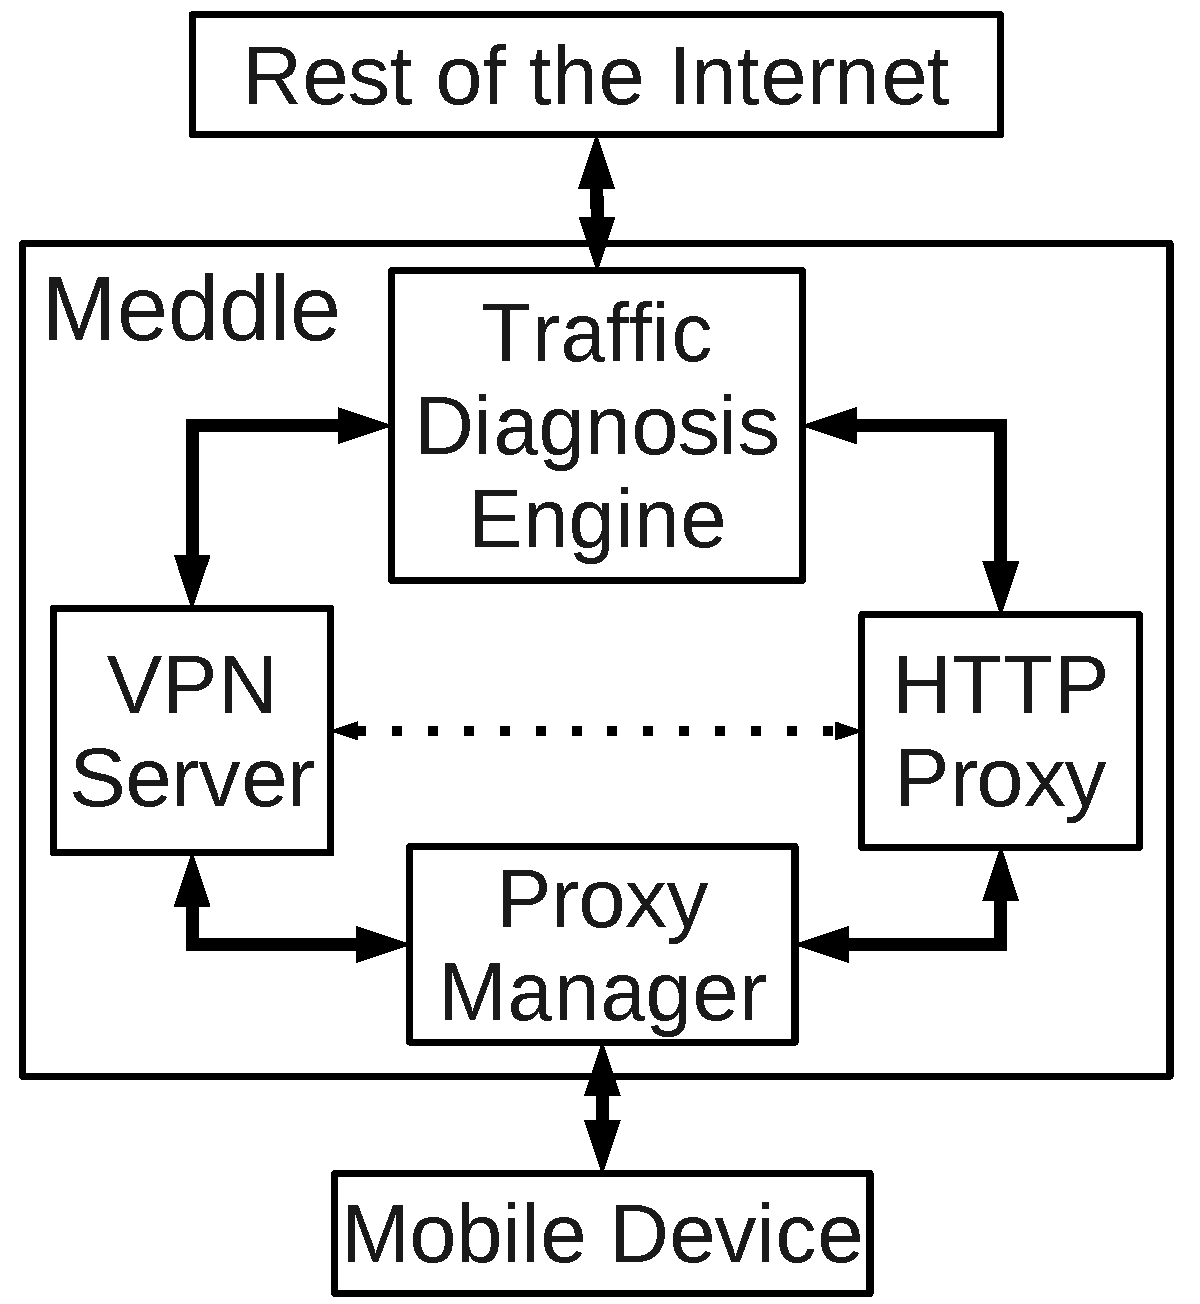
\includegraphics[width=2in]{figures/Meddle-Design.pdf}
\caption{Figure showing traffic redirection and flow of traffic through VPN and HTTP proxy}
\label{fig:architecture}
\end{figure}

Architecture as shown in Figure~\ref{fig:architecture}.

Explain two Proxies, one VPN and other HTTP.

Explain how each goal is met and why we need two proxies. 

The role of the VPNs Proxy.
VPNs allow tunnel everything (all IPv4 traffic). 
All IPv4 traffic can be monitored and controlled on the middlebox. 

The role of HTTP Proxy.
Check ISP interference.
What 
How tripwires are implemented. 


Though deployment of proxies appears to be straighforward they come with challenges that need to be addressed to make the solution practical and feasible. 
We now describe how we addressed these challenges.

\subsubsection{Configuration requirements.}

VPNs on mobile devices do not inherently tunnel all the Internet traffic.
However, mobile devices support features that can be built on to enable tunneling of all Internet traffic. 

All iOS devices (version 3.0 and above) support \textit{VPN On-Demand}, which forces traffic for a specified set of domains to use VPN tunnels. 
To ensure all possible destinations match this list, we exploit the fact that iOS uses suffix matching to determine which connections should be tunneled; accordingly, we specified the domain list as the set of alphanumeric characters (a-z, 0-9, one character per domain). 
Android version 4.2 and above supports an \textit{Always On VPN} connection that provides the same functionality; for Android version 4.0 and above there is an app API that allows apps to manage VPN tunnels. 
We support both options.
Both iOS and Android support VPN connections using the IPSec standard, This means we can implement our VPN proxy server using free and open-source code from Strongswan~\cite{strongswan}. 

\tbd{Tripwire}


\subsection{Existing Deployment}

Where is this currently deployed?

What is the objective of this deployment?

Who are the ones signed up?

What was the incentive given?

\subsection{VPN Overheads}

%\begin{packedenumerate}
%\item 

\noindent\textbf{Increase in Network Latency.}
We measured 50 VPN-connection establishment times  on both iOS (iPhone 5 / iOS 6.1) and Android (Galaxy Nexus /
Android 4.2), for \wifi{} and cellular connections. 
The \meddle server was running on a university network. 
For Android (using IKEv2), the maximum establishment time was 0.81 seconds on \wifi{} and 1.59 seconds on cellular. 
For iOS (using IKEv1), the connection takes longer due to the older protocol version: we observe a maximum of 2 seconds on \wifi{} and 2.18 seconds on cellular. 
Because each VPN session supports many flows, the amortized cost of connecting is  small. 
\tbd{Cite results from latency to home gateways based on DSL results in PAM and IMC.}
\tbd{Address comments in conext review on latency}

%\item 
\noindent\textbf{Increase in Power Consumption.}
Mobile devices expend additional power to establish, maintain and encrypt data for a VPN tunnel. 
To evaluate the impact on battery, we used a power meter to measure the draw from a Galaxy Nexus running Android 4.2. 
We run 10-minute experiments with and without the VPN enabled. 
For each experiment, we used an activity script that included Web and map searches, Facebook interaction, e-mail and video
streaming. 
The VPN leads to a 10\% power overhead. \tbd{min, max, median for results given by dave}. 
For iOS devices, we relied on the battery readings provided by iOS because we cannot attach a power meter directly to the battery.
We again found an approximately 10\% power overhead of using VPNs when we drained a fully charged battery while performing the operations performed during the tests for Android devices.  

%\item 
\noindent\textbf{Increase in Traffic Volume.}
\meddle relies on IPsec for datagram encryption, thus there is an encapsulation overhead for each tunneled packet. 
To evaluate this overhead, we use 30 days of data from 25 devices that to compare encapsulated and raw packet sizes. 
We observe a maximum encapsulation overhead of 12.8\% (average approximately 10\%). 
Within the scope of the traffic monitoring experiments performed with \meddle, the impact of this overhead is negligible. 
However, in case of experiments with a limited cellular data plan, this overhead must be taken into account
%\end{packedenumerate}

\subsection{Limitations}

\noindent\textbf{At most one tunnel.}
\tbd{Not true for http proxy}
Currently iOS and Android support exactly one VPN connection at a time. 
This allows \meddle{} to measure traffic over either \wifi or cellular interfaces, but not both at once.
The vast majority of traffic uses only one of these interfaces, and that interface uses the VPN

\noindent\textbf{Proxy location.} 
When traffic traverses the \meddle{} box, destinations will see the \meddle{} box address, not the device IP, as the source. 
This might impact services  that customize (or block access to) content according to IP address (e.g., in case of localization). 
A solution to this problem is to use a \meddle{} instance with an appropriate IP address

\noindent\textbf{ISP support.}
Some ISPs block VPN traffic, which prevents access to our current \meddle implementation. 
We note that few ISPs block VPN traffic, and there is an incentive not to block VPN traffic to support enterprise clients.

\noindent\textbf{IPv6.}
\meddle{} cannot be currently used on networks using IPv6 because IPv6 is not fully supported by mobile devices. 
Indeed, we observe that though iOS and Android support IPv6 they currently do not support IPv6 traffic through VPN tunnels

\noindent\textbf{MPTCP?.}
%\noindent\item \textbf{Wi-Fi Gateways powered by Cellular Modems.}


\subsection{Costs}

\noindent\textbf{Deployment and Running Costs}

\noindent\textbf{Trust Provider}

\subsection{Incentive for End-user Deployment}

\noindent \textbf{Deploy on Home Gateway.}
This is why we need the single machine constraint. 

\noindent \textbf{Packet Filtering.}
Custom ad blocks. Protect against data leaks. 

\noindent \textbf{Security from untrusted Wi-Fi APs.}

\noindent \textbf{Modular Architecture for Offloading Activities.}

%%% Local Variables: 
%%% mode: latex
%%% TeX-master: "meddle-main"
%%% End: 
